\chapter{Application}
\label{chap:app}
% * why?
% * current results/techniques
%%%%%%%%%%%%%%%%%%%%%%%%%%%%%%%%%%%%%%%%%%%%%%%%%%%%%%%%%%%%%%%%%%%%%%%%%%%%%%%%

% * Growing interest, application, ...
% * to show its working apply our method to energy transfer and absorption spectra of molecular aggregat
% * DEF. Molecular aggregat: assemblies of monomers (molecules, atoms, ...), where monomers largely keep individual properties
%     * interaction leads to collevcitve phenomena
%     * for sake of clarity: monomer = molecule in our notation
% * Non-markovian effects
% * demonstrate applicability to systems of recent interest


%%%%%%%%%%%%%%%%%%%%%%%%%%%%%%%%%%%%%%%%%%%%%%%%%%%%%%%%%%%%%%%%%%%%%%%%%%%%%%%%
\section{Basic Model}
\label{sec:app.model}
% * assumptions
% * Frenkel excitons
%
% FIXME Too many subsections?
% TODO Experimental setup, necessary for app.model.exciton
% TODO product initial state ok, vertical Frank-Condon transition
%%%%%%%%%%%%%%%%%%%%%%%%%%%%%%%%%%%%%%%%%%%%%%%%%%%%%%%%%%%%%%%%%%%%%%%%%%%%%%%%

%%%%%%%%%%%%%%%%%%%%%%%%%%%%%%%%%%%%%%%%%%%%%%%%%%%%%%%%%%%%%%%%%%%%%%%%%%%%%%%%
\subsection{The Aggregat Hamiltonian}
\label{sub:app.model.hamiltonian}

% GENERAL MOLECULE
% ---------------
% ✔ molecular Hamiltonian, Born Oppenheimer approx (large difference in mass)
%     => seperation of time scales,
% ✔ split into electronic and vibrational degrees of freedom
% ✔ in aggregat further vibrational degrees of freedom: inter- and intramolecular as well as solvent
%
% FIXME Rename V_mn since we use it below for matrix elements

In the follwing chapter we treat molecular aggregats with a size in the order of magnitude from a few up to a hundred molecules.
Let us consider the latter composed of electrons and point-like nuclei quantum mechanically described by canonical-conjugated pairs of operators $(p_j, q_j)$ and $(P_j, Q_j)$ respectively.
The corresponding Hamiltonian is given by
\begin{equation}
  \opH{mol} = \opT{el} + \opT{nuc} + \opV{el-el} + \opV{nuc-nuc} + \opV{el-nuc}
  \label{eq:app.mol_hamil}
\end{equation}
% TODO More?
with the kinetic energies $T$ and appropriate Coulomb interactions $V$.
% TODO Really?
We drop possible contributions from internal spin degrees of freedom since they induce only negligible corrections for the systems under consideration.

The vast difference in masses of electrons and nuclei allows us to separate the dynamics of both into two individual parts using the Born-Oppenheimer approximation:
As electrons move on a much faster time scale they can respond to any changes in the nuclear arrangement almost instantaneously.
This amounts to including the motion of nuclei mediated by the Coulomb potential $\opV{el-nuc}$ only adiabatically when calculating the electron dynamics from \autoref{eq:app.mol_hamil}.
% TODO Is this clear and to the point?
Therefor we can reorganize the summands in \autoref{eq:app.mol_hamil} more appropriately to
\begin{equation}
  \opH{mol} = \opH{el}(\QQ) + \opT{nuc} + \opV{nuc-nuc},
  \label{eq:app.mol_hamil_bo}
\end{equation}
where the notation $\opH{el} = \opT{el} + \opV{el-el} + \opV{el-nuc}(\QQ)$ indicates that we regard the electronic Hamiltonian to depend only parametrically on the nuclear coordinates $\QQ$.
% FIXME Notice??
For the processes under consideration only the valence electrons need to be taken into account explicitly; others are included to the nucleon-part without further notice.


% FIXME In all possible combinations?
The same reasoning applies to the complete Hamiltonian of the aggregat, which besides contributions of the form~\ref{eq:app.mol_hamil} for each individual molecule contains intermolecular interactions between electrons and nuclei in all possible combinations.
Therefore it can rephrased similarly to \autoref{eq:app.mol_hamil_bo}
\begin{equation}
  \opH{agg} = \opH{el}(\QQ) + \opT{vib} + \opV{vib-vib},
  \label{eq:app.agg_hamil}
\end{equation}
Here we use the more general notion of vibrational degrees of freedom, which not only comprises the intra- and intermolecular nuclear coordinates, but also possible environmental degrees of freedom not belonging to the aggregat.
These appear for example when studying molecular compounds immersed in a liquid solvent.

% ELECTRONIC PART
% ---------------
% * Holstein model
% ✔ no exchange interaction due to seperation of molecules, no overlap (tight binding)
% ✔   => anti-symmetrization in Hartree anatz non necessary; product basis
% ✔      =>   H_el = Σ_ma ε_ma |φ_ma><φ_ma|  +  ½ Σ ...

The Born-Oppenheimer approximation allows us to analyse the electronic separately from the vibrational part of \autoref{eq:app.agg_hamil} for a fixed coordinate vector $\QQ$.
We split up the former into contributions for each individual electron
\begin{equation*}
  \opH{el} = \sum_m H_m^\mathrm{(el)} + \frac{1}{2} \sum_{m,n} U_{mn}^\mathrm{(el-el)},
\end{equation*}
where $H_m^\mathrm{(el)}$ contains the $m$\th electron's kinetic energy as well as its coupling to the vibrational degrees of freedom and $U_{mn}$ is simply the Coulomb interaction between the $m$\th and $n$\th electron.
The \quotes{free} Hamiltonians $H_m^\mathrm{(el)}$ define distinct electronic states by
\begin{equation*}
  H_m^\mathrm{(el)}(\QQ) \varphi_{ma} (q, \QQ) = \epsilon_{ma}(\QQ) \varphi_{ma} (q, \QQ)
\end{equation*}
for each given environmental configuration $\QQ$.
The index $m$ runs over all electrons under consideration and $a$ is used to label the individual states, which we assume to be ordered by the corresponding energies.
Similar to the Hartree-Fock method we build up an expansion basis for the total electronic state by a product ansatz
\begin{equation}
  \phi_{\vec a}(\qq, \QQ) = \prod_m \varphi_{m, a_m}(q_m, \QQ),
  \label{eq:app.product_states}
\end{equation}
which in general needs to be anti-symmetrized to fulfill the Pauli exclusion principle.

If there is at most one valence electron per molecule we need to take into consideration, which is furthermore tightly bound, then the situation simplifies dramatically:
In this case the spreading of the single-electron states $\ket{\varphi_{ma}} = \ket{m, a}$ is small compared to the distance between two molecules; we can neglect the overlap $\braket{m, a}{n, b}$ for different molecules $m \neq n$.
Consequently \autoref{app.product_states} yields a complete basis for the electronic degrees of freedom.
We also have the following representation for the Hamiltonian~\ref{eq:app.agg_hamil}% FIXME Formula!
\begin{equation}
  \opH{el} = \sum_{m, a} \epsilon_{m, a} \, \ket{m, a}\bra{m, a} + \frac{1}{2}\sum_{m,n,a,b,a',b'} U_{mn}(aa', bb') \, \ket{m,a; n,b}\bra{m,a'; n,b'}
  \label{eq:app.agg_hamil_basis}
\end{equation}
with the matrix elements of the Coulomb interaction\footnote{%
  % TODO Mutual enough?
  This does not include the exchange interaction, since we assume a vanishing mutual overlap for the electrons.
}
\begin{equation*}
  U_{mn}(aa', bb') = \bra{m,a; n,b} U_{mn} \ket{m,a'; n,b'}.
\end{equation*}
% TODO Is this correct?
Note that all terms in \autoref{eq_app.agg_hamil_basis} still depend on vibrational coordinates.
For example the matrix elements $U_{mn}(aa'; bb')$ is influenced by the distance between the $m$\th and $n$\th molecule, while the electronic eigenenergies $\epsilon_{m, a}$ primarily depend on the positions of other electrons belonging to the same molecule.

%%%%%%%%%%%%%%%%%%%%%%%%%%%%%%%%%%%%%%%%%%%%%%%%%%%%%%%%%%%%%%%%%%%%%%%%%%%%%%%%
\subsection{The Exciton Model}
\label{sub:app.model.exciton}
% ✔ beside electronic ground state only first excited singlet state φ_m^g, φ_m^e for each molecule
% ✔   => effective 2 level system
%     * ok if only one S_1 state is initially excited and all first-level energies are same order of magnitude
% ✔ different contributions to interaction term; Heitler-London approximation (p.370)
% ✔   => Interaction term gives only "hopping" contributions (resonant excitation energy transfer)
%     => if we start with single excitation, we remain in the single-excitation Hilbert space
% ✔   => basis vectors |π_n> = |φ_n^e> Π_i≠n |φ_i^g> => single exciton state
%     * need ground state |0> = Π_i |φ_i^g> as well due to dissipation
%     * multi-exciton states for nonlinear stuff
%     * interaction matrix elements can be calculated from center-of-mass coordinate of molecule and Coulomb interaction
%        => more details (dipole approximation, etc.) in spectrum-section
%
% TODO Dipol-Dipol interactoin approximation (p.372)

% TODO Good? Position of footnote?
% FIXME I am too long!!!
In order to describe the experimental setting described in the introduction we do not need to consider the complete electronic Hamiltonian~\ref{eq:app.agg_hamil_basis}:
if only a single valence electron is initially in the lowest excited state $S_1$ above its ground state $S_0$\footnote{%
  Note that $S_0$ describes the lowest energy state of the valence electron with all other electrons of the molecule fixed, not to be confused with the atomic ground states.
}
and if the various transition energies are in the same order of magnitude, then it is sufficient to take only the $S_0$ state $\ket{m, 0}$ as well as the first excited stated $\ket{m, 1}$ for each molecule into account.
% FIXME Is charged induced transition a word?
Under these circumstances the matrix elements $U_{mn}(aa', bb')$ can be classified with respect to a few physical processes such as electrostatic interactions or charge-induced transitions.
But most important is the resonant contribution $U_{mn}(01; 10)$ (and its inversion $U_{mn}(10; 01)$) describing a $S_0 \to S_1$ excitation for the $m$\th electron induced by a  $S_0 \to S_1$ transition at the $n$\th molecule.
In the following we neglect all but the last class of processes, which is frequently called Heitler-London approximation.

Restricting the allowed electronic states to the two lowest energy levels has a remarkable interpretation in terms of quasi-particles:
The product
\begin{equation}
  \ket{m} = \ket{m, 1} \prod_{n \neq m} \ket{n, 0}
  \label{eq:app.exciton_state}
\end{equation}
% TODO What about gorund state?
% FIXME Too much due to, therefore,...
describes an excited electron localized in the vicinity of the $m$\th molecule, which we refer to as an exciton of the electronic system.
Due to the Heitler-London approximation our adiabatic Hamiltonian~\ref{eq:app.agg_hamil_basis} conserves the number of excitons.
Therefore an initial state $\ket{m}$ (or linear combinations thereof) always remains in the one-exciton Hilbert space $\HH^{(1)}$.
% TODO WHY???
The interaction matrix elements
\begin{equation*}
  V_{mn} = V_{nm} = \bra{m, 0; n, 1} U_{mn} \ket{m, 1; n, 0}
\end{equation*}
allow us to express the restriction of $\opH{el}$ to $\HH^{(1)}$ as
\begin{equation*}
  \opH{el}^{(1)}(\QQ) = \sum_m \epsilon_m(\QQ) \ket{m}\bra{m} + \sum_{m,n} V_{mn}(\QQ) \ket{n}\bra{m}.
\end{equation*}
% FIXME Second sentence strange...
For the rest of this section we assume the $V_{mn}$ to be independent of vibrational degrees of freedom; a more general treatment poses no further difficulties.\\

% VIBRATIONAL PART
% ----------------
% ✔ include dynamica

% FIXME Too much "degrees of freedom"
Up to this point we have neglected the dynamical evolution of the vibrational environment, which is essential in a complete description of a molecular aggregat.
% TODO REALLY? WHY?
In common settings for the physical systems under consideration a harmonic approximation is sufficient to obtain a realistic model.
There are two reasons for this:
First of all most proteins disintegrate at temperatures much higher than room temperature; therefore thermal excitation only leads to small energy gains for each vibrational degree of freedom.
The other mechanism for driving the environment is dissipation of the electronic system.
But the latter is small compared to the vast number of vibrational degrees of freedom and energy typically spreads evenly across the environment.
We can thusly assume that all $Q_\lambda$ experience only a small displacement from their equilibrium positions, which we set to $Q_\lambda = 0$.

% TODO More?
As a consequence both $\opV{vib-vib}(\QQ)$ and $\epsilon_m(\QQ)$ can be expanded in a Taylor series neglecting all but the first non-trivial term.
To alleviate notation we further assume that each vibrational degree of freedom only couples to one specific exciton.
This leads to exactly the microscopical model presented in \autoref{sec:nmqsd.model}: a bath of harmonic oscillators linearly coupled to the electronic system
\begin{align*}
  \opH{agg} =
  \sum_m \epsilon_m(0) \ket{m}\bra{m} + \sum_{m,n} V_{mn} \ket{m}\bra{n} + \sum_{m, \lambda} \omega_{m, \lambda} \adj{A}_{m, \lambda} A_{m, \lambda} \\
  + \sum_{m, \lambda} g_{m, \lambda} \ket{m}\bra{m} \otimes \left( \adj{A}_{m, \lambda} + A_{m, \lambda} \right),
\end{align*}
where $A_{m, \lambda}/\adj{A}_{m, \lambda}$ are ladder operators corresponding to the $\lambda$\th vibrational mode coupling to the $m$\th exciton.

% TODO ε_m(0) = ε_m ... site energy; optical transition energy at the equilibrium configuration of env. phonons associated with S_0 state
% V_mn electronic coupling strength


%%%%%%%%%%%%%%%%%%%%%%%%%%%%%%%%%%%%%%%%%%%%%%%%%%%%%%%%%%%%%%%%%%%%%%%%%%%%%%%%
\section{Transfer Dynamics }
\label{sec:app.fmo}
%%%%%%%%%%%%%%%%%%%%%%%%%%%%%%%%%%%%%%%%%%%%%%%%%%%%%%%%%%%%%%%%%%%%%%%%%%%%%%%%

%% FMO Structure plots %%%%%%%%%%%%%%%%%%%%%%%%%%%%%%%%%%%%%%%%%%%%%%%%%%%%%%%%%
\begin{figure}[t]
  \centering
  \begin{subfigure}[t]{.6\textwidth}
    \centering
    \includegraphics[width=.8\textwidth]{img/fmo_monomer.png}
    % FIXME Better caption
    % FIXME Higher dpi
    \caption{%
      Spatial arrangement
    }
    \label{fig:app.monomer_full}
  \end{subfigure}
  \begin{subfigure}[t]{.3\textwidth}
    % FIXME Colors
    \centering
    \definecolor{qqttcc}{rgb}{0,0.2,0.8}
    \definecolor{ffqqzz}{rgb}{1,0,0.6}
    \definecolor{ffqqqq}{rgb}{1,0,0}
    \definecolor{qqcccc}{rgb}{0,0.8,0.8}
    \definecolor{ffzzqq}{rgb}{0.6,0.6,0.6}
    \definecolor{qqffqq}{rgb}{0,1,0}
    \begin{tikzpicture}[line cap=round,line join=round,>=triangle 45, xscale=.5, yscale=.014]
      \draw[->,color=black] (0,-55.09) -- (0,409.79);
      \foreach \y in {0, 100, 200, 300}
      \draw[shift={(0,\y)},color=black] (2pt,0pt) -- (-2pt,0pt) node[left] {\footnotesize $\y$};
      \draw[color=black] (-2.30, 180) node[rotate=90] {$\epsilon_m$ [$cm^{-1}$]};
      \clip(-0.38,-55.09) rectangle (5.9,409.79);
      \draw [line width=2pt, color=red] (0.17,180)-- (1.17,180);
      \draw [line width=2pt,color=qqffqq] (1.39,300)-- (2.39,300);
      \draw [line width=2pt,color=ffzzqq] (3.63,400)-- (4.63,400);
      \draw [line width=2pt,color=qqcccc] (2.89,250)-- (3.89,250);
      \draw [line width=2pt,color=orange] (3.85,210)-- (4.85,210);
      \draw [line width=2pt,color=ffqqzz] (2.57,80)-- (3.57,80);
      \draw [line width=2pt,color=qqttcc] (1.81,0)-- (2.81,0);
      \draw [line width=1pt] (0.74,189.05) -- (1.8,284.18);
      \draw [line width=1pt] (4.13,384.05) -- (3.43,259.34);
      \draw [line width=1pt] (4.13,384.05) -- (4.32,221.85);
      \draw [line width=1pt] (3.4,233.65) -- (3.04,87.89);
      \draw [line width=1pt] (3.03,66.68) -- (2.39,9.1);
      \draw [line width=1pt] (4.32,193.38) -- (3.21,87.14);
      \draw [line width=1pt] (1.95,283.23) -- (2.25,9.1);
      \begin{scriptsize}
        \draw[color=red] (0.68,168) node {180};
        \draw[color=qqffqq] (1.90,288.0) node {300};
        \draw[color=ffzzqq] (4.15,388.0) node {400};
        \draw[color=qqcccc] (3.4,238.0) node {250};
        \draw[color=orange] (4.4,198.0) node {210};
        \draw[color=ffqqzz] (3.05,68.0) node {80};
        \draw[color=qqttcc] (2.3,-12.0) node {0};
      \end{scriptsize}
    \end{tikzpicture}
  % FIXME LABEL AND CAPTION
    \caption{%
      Site energies
    }
    \label{fig:app.site_energies}
  \end{subfigure}
  \caption{%
    Spatial and energetic structure of the simplified FMO-monomer with seven BChls; the coloring and numbering is used throughout this section.
    \textbf{(a)} Was created using the molecular visualization system \textsc{PyMOL} based on the \textsc{PDB} entry \textsc{3eni} \cite{pymol,TrCaBl09_fmo_structure}.
    \textbf{(b)} Shows the site energies of \emph{Chlorobaculum tepidum} \cite{AdRe06_fmo}; lines indicate dominant couplings leading to the two distinct transport channels.
  }
\end{figure}
%%%%%%%%%%%%%%%%%%%%%%%%%%%%%%%%%%%%%%%%%%%%%%%%%%%%%%%%%%%%%%%%%%%%%%%%%%%%%%%%

% ✔ why FMO?
% ✔   * small size: typical model system photosyntetic exciton energy transfer
% ✔   => function: transfer electronic excitation energy from the chlorosome (light harvesting antenna) to the photosyntetic reaction center in green sulfur bacteria
% ✔   * 90s: electronic quantum coherence observed; only recently realized: key feature in nearly unit yield transport
%     * role of coherence: avoid local energetic traps; aid efficient trapping of electronic energy by the pigments facing the reaction center \cite{IsFl09_fmo}
%        => exciton superposition states (formed during fast excitation event) allow the excitation to "reversibly sample all posible paths"
%        => efficient directing the energy transfer to find the most effective sink for the excitation energy \cite{EnCaRe07_photosyn}
% ✔      => efficiency beyond classical sampling-by-hopping
% ✔   * before that: semiclass. hopping (Förster theory)

As a first exemplary application of our hierarchical equations of motion we study energy transfer in the Fenna-Matthews-Olson (FMO) complex found in low-light adapted green sulfur bacteria.
This protein complex plays a crucial role in connecting the light harvesting antenna (chlorosome) to the photosyntetic reaction center, where the absorbed solar energy is converted to a charge gradient.
% FIXME Quantumness???
The vast amount of literature on the subject is not only by virtue of its relatively small size---making it an ideal model for numerical investigation---but particularly due to the strong influence of quantum mechanical effects on the transfer, even at physiological temperature.
Only lately Engel et al.\ as well as Ishizaki-Fleming demonstrated that the FMO complex achieves its remarkable almost-unit efficiency by coherent exciton motion instead of classical hopping described by Förster theory \cite{EnCaRe07_fmo,IsFl09_fmo}. \\



% ✔ structure: 3 identical subunits, called monomers
% ✔ these consist of eight BChl molecules
% ✔   * here we focus on one monomer (as shown in \cite{RiRoSt11_fmo_trimer} reasonable approximation due to small coupling between monomers
%     * energy transfer between monomers via resonacne Coulomb interaction (weak!)
% ✔ site energies and electronic coupling depend on protein environment, different values in literature;
%     ✔ here: Chlorobaculum tepidum, from \cite{AdRe06_fmo}A
%     ✔ data was obtained how???
% ✔ no detailed info about specral density for FMO complex
%     ✔ assume independent, but equivalent for each BChl, data from \cite{IsFl09_fmo}
%     * detailed study in \cite{RiRoSt11_fmo}

The FMO protein complex is subdivided into three identical monomers, each comprising eight bacteriochlorophyll pigments (BChls).
% FIXME +3
In contrast to the first seven BChls, the eighth was only discovered in recent years due to its rather weak coupling to the remaining BChls and instability during the isolation procedure in experiments \cite{TrCaBl09_fmo_structure,ScMuEl10_eighth}.
As the main goal here is to show the applicability and reliability of our hierarchical equations of motion we ignore BChl number eight in what follows---this simplified model has been investigated thoroughly with a vast array of methods.
For the same reason, we also restrict our attention to an individual monomer: as shown by Ritschel et al.\ such a limitation is reasonable for the short time scales under consideration as the intermonomeric interaction strength is rather weak.

In \autoref{fig:app.monomer_full} we display the spatial structure and numbering of the BChls in single a monomer.
The BChls 1 and 6 are situated in the vicinity of the light harvesting antenna and receive excitation energy captured, while BChl 3 acts as energy sink.
As both site energies $\epsilon_n$ and electronic coupling strengths $V_{mn}$ depend on the protein environment, different values for different species can be found in the literature.
%> FIXME Where to put electronic coupling
Here we use the data obtained from optical spectroscopy in \emph{Chlorobaculum tepidum} \cite{AdRe06_fmo}, see \autorefs{fig:app.site_energies} and~\ref{fig:app.fmo_ishfl}.
Although the spectral density may be important for the details of the excitation transfer, no comprehensive information on this matter is available at present.
Good agreement with experiments on \emph{Prosthecochloris aesturaii} was achieved \cite{ReScEn08_fmo_spectral_density} under the semi-empirical assumption that each exciton couples to an independent environment with a Drude spectral density
\begin{equation}
  J(\omega) = \frac{2 \lambda}{\pi} \frac{\gamma\omega}{\omega^2 + \gamma^2},
  \label{eq:app.drude}
\end{equation}
with reorganization energy $\lambda = 35\,\mathrm{cm^{-1}}$ and relaxation time $\gamma^{-1} = 50\,\mathrm{fs}$.\\



%% Single Page with Transfer @77K %%%%%%%%%%%%%%%%%%%%%%%%%%%%%%%%%%%%%%%%%%%%%%
\begin{figure}[p]
  \centering
  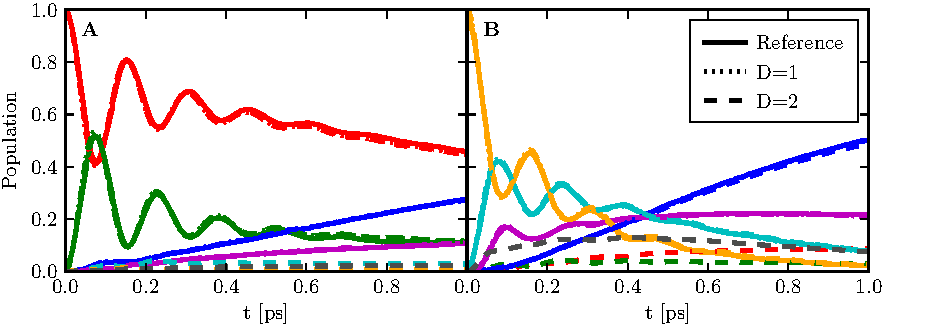
\includegraphics{img/fmo_ishfl}
  % FIXME Reference to color encoding?
  \caption{%
    \label{fig:app.fmo_ishfl}
    Exciton transfer of the simplified FMO-monomer with seven BChls at 77\,K using our stochastic hierarchical equations up to first~(doted) and second order~(dashed) averaged over 10000 trajectories.
    For comparison the solid line shows the results of Ishizaki and Fleming~\cite{IsFl09_fmo}, which were obtained in the HEOM approach.
    Population for BChls 1--4 \textbf{(A)} and BChls 3--6 \textbf{(B)} with initial excitation on site 1 and 6 respectively.
    The inset displays a purely electronic system without coupling to the vibrational degrees of freedom.
    Details on parameters can be found in \autoref{sec:coth.fmo}.
  }

  \vspace{.3cm}
  \centering
  % FIXME Run again, timescale is not right
  \begin{subfigure}[b]{0.3\textwidth}
    \includegraphics[width=\textwidth]{img/fmo_transfer_0.png}
    \caption{%
      $t = 0.00 \, \mathrm{ps}$
    }
  \end{subfigure}
  \begin{subfigure}[b]{0.3\textwidth}
    \includegraphics[width=\textwidth]{img/fmo_transfer_1.png}
    \caption{%
      $t = 0.2 \, \mathrm{ps}$
    }
  \end{subfigure}
  \begin{subfigure}[b]{0.3\textwidth}
    \includegraphics[width=\textwidth]{img/fmo_transfer_2.png}
    \caption{%
      $t = 0.50 \, \mathrm{ps}$
    }
  \end{subfigure}

  \begin{subfigure}[b]{0.3\textwidth}
    \includegraphics[width=\textwidth]{img/fmo_transfer_3.png}
    \caption{%
      $t = 1.00 \, \mathrm{ps}$
    }
  \end{subfigure}
  \begin{subfigure}[b]{0.3\textwidth}
    \includegraphics[width=\textwidth]{img/fmo_transfer_4.png}
    \caption{%
      $t = 2.00 \, \mathrm{ps}$
    }
  \end{subfigure}

  \caption{%
    \label{fig:app.fmo_transport_pretty}
    Same as \autoref{fig:app.fmo_ishfl} B.
    The intensity of each molecule represents the population of the associated exciton state.
    For the sake of clarity we do not show the full molecular structure.
  }
\end{figure}
%%%%%%%%%%%%%%%%%%%%%%%%%%%%%%%%%%%%%%%%%%%%%%%%%%%%%%%%%%%%%%%%%%%%%%%%%%%%%%%%

\Autoref{fig:app.fmo_ishfl} shows the results of our calculations at cryogenic temperature $T=77\,\mathrm{K}$ using our stochastic hierarchy as well as the established \HEOM-results of Ishizaki and Fleming \cite{IsFl09_fmo}.
Both initial excitations move remarkably fast and directed---and up to $t=700\,\mathrm{fs}$ in a quantum-coherent, wavelike fashion---toward the energy sink at BChl 3.
However, the final population of the latter is only about half as large on the left hand side due to the relatively high site energy of BChl 2.
This prolongs the lifetime of an exciton-state on BChl 1 significantly.
It has been conjecture that this barrier is partly responsible for the high yield of the FMO-complex \cite{IsFl09_fmo}.
Indeed, the relatively small energy gap $\Delta\epsilon = 180\, \mathrm{cm^{-1}}$ between the first and third BChl cannot prevent back-transfer due to thermal excitation from the latter along this channel.
The larger gap of $\Delta\epsilon = 300\,\mathrm{cm^{-1}}$ between the second and the third suppresses depopulation much more efficiently.
This is exactly where quantum effects influence the operation significantly:
Delocalization helps to overcome the resulting subsidiary energetic minima at BChl 1 much quicker than a classical hopping-excitation could.

No such initial \quotes{energy barrier} exists for the transport starting BChl 6, therefore, the excitation-population at molecules 3 and 4 increases up to $t = 1\,\mathrm{ps}$.
For even longer times, all other sites have only vanishing probability left as shown in \autoref{fig:app.fmo_transport_pretty}.

In the inset to \autoref{fig:app.fmo_ishfl} we also show the dynamics for a purely electronic system:
As expected the population-probability shows a purely oscillatory behavior with no effective excitation transport, thus emphasizing the importance of vibrational degrees of freedom in the exciton energy transfer.

Remarkably, the results of first and second order in our stochastic hierarchy are almost indistinguishable from each other and agree very well the reference.
% FIXME Is this a good idea?
Calculations including one more order (not shown) verify, that the second order is already enough to obtain convergence in these parameter regimes.
% FIXME Really?
As we show in \autoref{sec:coth.fmo}, the dominant exponential bath mode is given by\footnote{%
  Recall our notation $\alpha(t) = g \exp[-\gamma\abs{t}]$.
}
$g \approx (2916 - \ii 3716) \, \mathrm{cm^{-2}}$ and $\gamma \approx 106\,\mathrm{cm^{-1}}$.
Therefore the proposed truncation condition $\sqrt{g} \ll k \gamma$, which for the given parameters reads $83 \ll 106 k$, might be too restricting, yet.

That we do not obtain complete agreement in \autoref{app.fmo_ishfl} A has the following reason:
The parameter $g$ of the second bath mode (a low temperature correction term) remains real.
% FIXME Due to Drude; only one Pole, not discontinous at zero!
Therefore, the complete bath correlation function, which is simply the sum of both modes, obtains a non-vanishing imaginary part at $\alpha(0)$ due to truncating the infinite Matsubara expansion.
But since $\alpha$ is related to our driving processes $\ZZ$ by $\alpha(t-s) = \E[Z_t \ZZ_s]$, we cannot treat such an unphysical bath correlation function exactly.
% FIXME Picture?
Therefore we included an additional, almost-Markovian mode with purely imaginary $g$, such that $\Im\alpha(t)$ goes smoothly to zero as $t \to 0$ while changing $\alpha$ as little as possible---the details may be found in the appendix.\\



%% MevsPhi plot %%%%%%%%%%%%%%%%%%%%%%%%%%%%%%%%%%%%%%%%%%%%%%%%%%%%%%%%%%%%%%%%
\begin{figure}[p]
  \centering
  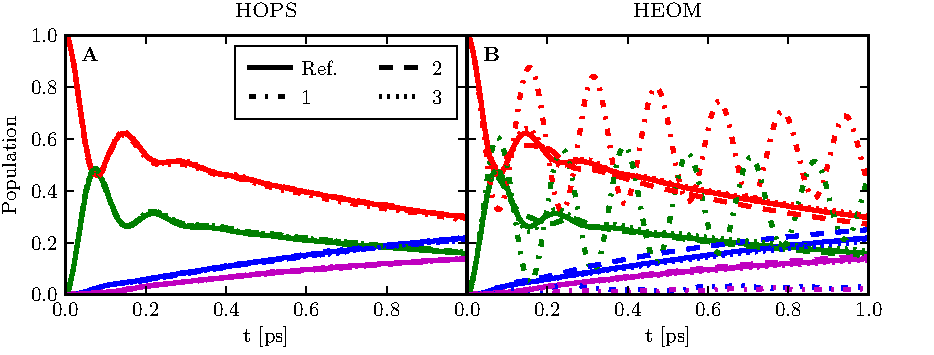
\includegraphics[width=\columnwidth]{img/fmo_mevsphi}
  \caption{%
    Exciton transfer of the simplified FMO-monomer at 300\,K and internal convergence check of the hierarchies. Solid lines are results from \cite{IsFl09_fmo}.\\
    \textbf{(A)} Stochastic hierarchy with 10000 realizations and orders 1--3.\\
    \textbf{(B)} Same sets of parameters, but calculated in the \HEOM formalism with truncation at orders 1, 2 and 5 using \textsc{PHI} \cite{StSc12_heom}.\\
    % FIXME Dashed lines same but 50000 realizations
    \textbf{(C)} The deviation of the stochastic hierarchy with respect to its third order result. Dotted lines indicate the maximum value over time. The starred curves correspond to a larger sample size of 50000 realizations.\\
    \textbf{(D)} Same as (C), but for the \HEOM calculation. Here, the reference is the fifth order result.
  }
  \label{fig:app.fmo_mevsphi}
\end{figure}
%%%%%%%%%%%%%%%%%%%%%%%%%%%%%%%%%%%%%%%%%%%%%%%%%%%%%%%%%%%%%%%%%%%%%%%%%%%%%%%%

The exciton dynamics at physiological temperature in \autoref{fig:app.fmo_mevsphi} shows a similar qualitative behavior.
However, the transfer is less efficient and directed as decoherence leads to a much stronger smearing of the excitation over all BChls, even the ones not shown in this picture.
For the same reason, the wave-like motion only lasts up to $t \approx 400\,\mathrm{fs}$.
Notwithstanding, at $t = 1\,\mathrm{ps}$ the population of the relevant, third BChl is $0.2$---still about two-thirds of the result at cryogenic temperature---and increases further.

This time, our stochastic hierarchical equations of motion reproduce the results of Ishizaki-Fleming almost exactly even with just one order.
In contrast to the $T = 77\,\mathrm{K}$ result, there is no pronounced offset, because the imaginary part of $\alpha(0)$ is insignificantly small
% FIXME Fill in alpha
\begin{equation*}
  \alpha(t) = \dots.
\end{equation*}
Again, we postpone the calculations to the appendix.
Nevertheless, the differences between first and second order are larger than for the former calculation.
% FIXME REally?
% FIXME Reference
Since the only distinction in the dominant bath mode is a larger coupling constant $g$, this strengthens our truncation condition~\ref{eq:}.

On the right hand side of \autoref{fig:app.fmo_mevsphi} B we carry out the same calculations using the \HEOM formalism \cite{StSc12_heom}.
Clearly, convergence with the number of hierarchies is much worse:
The first order calculations displays highly undamped oscillations and the second order is necessary to get the qualitative picture right.
We have found that a truncation at fifth order is necessary to correctly reproduce the coherent oscillations between 0\,fs and 300\,fs.

To check internal convergence of each method systematically, we proceed as follows:
First we define a measure for deviation of a given reduced density matrix $\rho(t)$, obtained from a numerical calculation, with respect to some reference $\rho^{\mathrm{ref}}(t)$ as
\begin{equation}
  A[\rho(t), \rho^\mathrm{ref}(t)] = \max\limits_n \left\vert \rho_{nn}(t) - \rho^{\mathrm{ref}}_{nn}(t) \right\vert.
  \autoref{eq:app.accuracy}
\end{equation}
since we confine our discussion to the populations of the exciton states $n$ given by $\rho_{nn}$.
As we are only interested in the convergence of a given method, the reference state is calculated using the same method and selected by increasing the truncation order $D$ until $A[\rho_{D}(t), \rho{D+1}(t)] < 10^{-3}$; then $\rho^{(ref)} = \rho_D$.
This amounts to $D=3$ for our \NMSSE-hierarchy and $D=5$ for $\HEOM$.
The accuracy of lower-order calculations with respect to the chosen reference is shown in \autoref{fig:app.fmo_mevsphi} C and D for the stochastic and the density hierarchy, respectively.

We already mentioned in the general discussion above that the first order's deviation of about 2\% is just barely visible in \autoref{fig:app.fmo_mevsphi} A.
In contrast, the same accuracy is obtained in the \HEOM-formalism not until we truncate the hierarchy at third order.
However, we notice an important difference in the two plots:
While the \HEOM-calculations show the largest discrepancy at the initial wave-like motion and then drop off by about an order of magnitude, the results from the stochastic hierarchy remain more or less constant after $t = 0.2\,\mathrm{ps}$.
This as well as the tremulous time-dependence indicate, that the error of the latter is due to stochastic effects and not caused by systematic deviation.
We check this statement by repeating the same calculations using a larger sample size---a start marks the corresponding results in \autoref{fig:app.fmo_mevsphi}.
Clearly, they show less deviation thus confirming our assertion.\\



In conclusion, the discussion above shows, that the hierarchical equations based on the nonlinear \NMSSE provide a highly efficient method to calculate exciton energy transfer dynamics in the FMO-complex.
We obtain almost perfect agreement for both, 77\,K and 300\,K, with the established results of Ishizaki and Fleming in first order calculations.
The discrepancy of these to higher order calculations is less than 1\% demonstrating very rapid convergence with respect to the truncation order.
Of course, such an accuracy is completely unnecessary for most investigations of biological systems.
The theoretical model itself is usually much less reliable due to approximations and experimental errors for the parameters involved.
Also, the improved numerical efficiency, due to a reduced number of auxiliary states\footnote{%
  In the case of a single bath mode, we have eight auxiliary states for $D=1$ compared to 330 for $D=4$.
}
and propagating Hilbert space vectors instead of density matrices, is more than compensated by the large sample size required.
However, the stochastic hierarchies' advantages really come to fruition when it comes to more realistic systems.
% FIXME Can we do this
For example, data from fluorescence line-narrowing measurements on \emph{Prosthecochloris aesturaii} indicate that realistic spectral densities are far more structured, requiring as much as 25 exponential modes
This amounts to 176 auxiliary states for $D=1$ compared to a tremendous number of 41 million states required by a fourth-order calculation.

%%%%%%%%%%%%%%%%%%%%%%%%%%%%%%%%%%%%%%%%%%%%%%%%%%%%%%%%%%%%%%%%%%%%%%%%%%%%%%%%
\section{Absorption Spectra}
\label{sec:app.spectra}
% * experimental setup
% * why not so good, but we still use them -> 2D spectroscopy
%%%%%%%%%%%%%%%%%%%%%%%%%%%%%%%%%%%%%%%%%%%%%%%%%%%%%%%%%%%%%%%%%%%%%%%%%%%%%%%%

%%%%%%%%%%%%%%%%%%%%%%%%%%%%%%%%%%%%%%%%%%%%%%%%%%%%%%%%%%%%%%%%%%%%%%%%%%%%%%%%
\subsection{NMSSE for Spectra}
\label{sub:app.spectra.nmsse}
% * why nmsse so good for this?

%%%%%%%%%%%%%%%%%%%%%%%%%%%%%%%%%%%%%%%%%%%%%%%%%%%%%%%%%%%%%%%%%%%%%%%%%%%%%%%%
\subsection{Results}
\label{sub:app.spectra.results}
% * other techniques
% * cool behavior of hierarchies
